\documentclass[a4paper,reqno]{amsart}
\usepackage{amssymb}
\usepackage{amsmath}
\usepackage{tikz}

\begin{document}

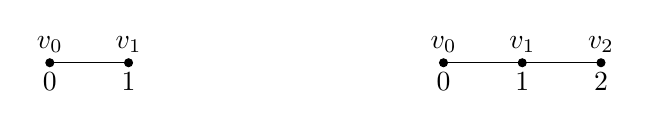
\begin{tikzpicture}
    \draw[fill] (0,0) circle(0.05) node[above]{$v_0$};
    \draw (0,0) node[below]{$0$};
    \draw[fill] (1,0) circle(0.05) node[above]{$v_1$};
    \draw (1,0) node[below]{$1$};  
    \draw (0,0)--(1,0);
    \begin{scope}[shift={(5,0)}]
     \draw[fill] (0,0) circle(0.05) node[above]{$v_0$};
      \draw (0,0) node[below]{$0$};
      \draw[fill] (1,0) circle(0.05) node[above]{$v_1$};
      \draw (1,0) node[below]{$1$}; 
      \draw (0,0)--(1,0);
      \draw[fill] (2,0) circle(0.05) node[above]{$v_2$};
      \draw (2,0) node[below]{$2$};
      \draw (1,0)--(2,0);
    \end{scope}
  \end{tikzpicture}

\end{document}